%!TEX root = ../cluster_semi.tex
\section{Evaluation}
\label{sec:evaluation}
To evaluate the performance of \name, we have conducted extensive experiments using real-world data collected from a top global online game service.
We first introduce the data set (Section~\ref{subsec:datasets}) and metrics (Section~\ref{subsec:evaluation_metrics}) used for the evaluation experiments.
% To demonstrate the overall performance of \name{} in detecting anomalies for KPI streams, 
Then, we compare the performance of \name{} with that of supervised learning based method such as Opprentice, and unsupervised learning based method including iForest and Donut (Section~\ref{subsec:overall-performance}).
Finally, to highlight the importance of semi-supervised learning, we compare \name{} with the combination of ROCKA and Opprentice (Section~\ref{subsec:effects_of_techniques}).
% Finally, we show how to tune aThld based on empirical experiments (Section~\ref{subsec:choose_threshold}).



% In this Section, we conduct some experiments to evaluate the performance of \name{}. First, we will introduce our KPI stream set. Then we will show the evaluation metrics and results for both ROCKA and CPLE. Finally, we show the effects of CPLE in \name{}.

\subsection{Data Set}
\label{subsec:datasets}

\begin{table*}
% \notes{Update after experiment is done}
\caption{Description of the new 81 KPI streams}
% \vspace{-0.5em}
\label{table:game-related-KPI}
\begin{center}
\begin{tabular}{| c | c | c | c | c |}
\hline
\textbf{KPI} & \textbf{\tabincell{l}{\# KPI \\streams}} & \textbf{\tabincell{l}{Interval \\(minute)}} & \textbf{\tabincell{l}{Length \\(month)}} &\textbf{\tabincell{l}{\#/percentage of anomalous \\data points per KPI stream}} \\ \hline
Latency & 19 & 5 & 1 & 150/1.7\% \\ \hline
\# online players & 58 & 5 & 1 & 72/0.83\% \\ \hline
Success rate & 4 & 5 & 1 & 84/0.97\% \\ \hline
\end{tabular}
\end{center}
% \vspace{-1.5em}
\vspace{-6 mm}
\end{table*}

We randomly pick 70 historical KPI streams for clustering and 81 new ones for anomaly detection from a top global online game service.
% We divide the above KPI streams into 
These KPI streams are of the most important three KPIs, including success rate, number of online players and latency.
Table~\ref{table:game-related-KPI} lists the detailed information of the 81 new KPI streams, including the number, interval and length of the KPI streams of each KPI. 
In addition, it also lists the averaged number and percentage of anomalous data points per KPI stream of each KPI, respectively. 

Note that the KPI streams of the same KPI may have very different shapes and thus belong to different clusters.
Therefore, experienced operators first manually group the 70 historical KPI streams into five clusters according to their shapes, and then classify the new 81 KPI streams into the five clusters.
This serves as the ground truth for clustering.

As mentioned in Section~\ref{subsubsec:preprocessing}, in this work we apply ROCKA to cluster KPI streams.
Based on the manual clustering results by operators, we find that ROCKA accurately groups \emph{all} the 70 historical KPI streams into the \emph{right} cluster.
In addition, ROCKA successfully classifies \emph{all} the 81 new KPI streams into the \emph{correct} cluster.

To evaluate the performance of anomaly detection methods, operators also manually label anomalous data points for the 81 new KPI streams, as well as the 5 historical KPI streams that are on cluster centroids (calculated using \ROCKA{}).
Note that we focus on anomaly detection on newly emerging KPI streams in this work, and thus
only the new 81 KPI streams are used for the following evaluation experiments.
Therefore, there is no need to manually labeling the remaining 65 historical KPI streams.
% 151 KPI streams (70 historical KPI streams and the 81 new ones).

As aforementioned, more than 6000 new KPI streams are produced per 10 days.
However, manually clustering and labeling anomalies for thousands of KPI streams is infeasible, considering the long period of KPI streams (one month).
Therefore, we randomly selected 151 KPI streams in our evaluation.
We believe that the 151 KPI streams are sufficient to evaluate \name{}'s performance.

% We obtain 86 well-maintained KPI streams, including success rate, statistics of players and latency three KPI types, which covers most of the curve types in the business from the most famous company in China. 
% The description of KPI streams is shown in TABLE~\ref{table:game-related-KPI}. 
% In practice, \emph{the KPI streams which belongs to the same type maybe have different shapes}. The experts of the company group these KPI streams into five clusters according to their shapes and label all the anomalies in the KPI stream set as groudtruth. All KPI streams have an interval of 5 minutes for about one month. The huge KPI stream set can ensure that we make an accurate assessment of the algorithm.

% Our experiments were conducted on a machine with Intel(R) Xeon(R) CPU E5-2630 v3 @ 2.40GHz and 64GB RAM.

% \begin{table*}
% \caption{Description of KPI streams}
% % \vspace{-0.5em}
% \label{table:game-related-KPI}
% \begin{center}
% \begin{tabular}{| c | r | r | r |}
% \hline
% \textbf{KPI type} & Latency & Statistics of players & Success rate \\ \hline
% \textbf{Number} & 22 & 60 & 4 \\ \hline
% \textbf{Interval (minute)} & 5 & 5 & 5 \\ \hline
% \textbf{Length (month)} & 1 & 1 & 1 \\ \hline
% \textbf{Average anomaly points} & 150/1.7\% & 72/0.81\% & 84/0.97\% \\ \hline
% \textbf{Noise} & Strong & Weak & Moderate \\
% \hline
% \end{tabular}
% \end{center}
% % \vspace{-1.5em}
% \end{table*}



\subsection{Evaluation Metrics}
\label{subsec:evaluation_metrics}
% For clustering, we use F-score to evaluate performance as discussed in ROCKA~\cite{lirobust}. 
% Also, some KPI streams maybe change their shapes because of the service changes or machine malfunctions which will result in that they are far away from any centroids. We call them outliers. We use a metric, \textbf{fraction of outliers} to show the percentage of outliers. Anomaly detection on these irregular shape outliers needs extra work. We ignore these KPI streams in clustering and anomaly detection evaluation simply in our experiments.

% For anomaly detection, most papers use point-wise metrics, but in real applications, the operators don't care about anomaly points but the whole anomaly segment. 
In real applications, the human operators generally do not care about the point-wise metrics. Therefore, we use a simple strategy following~\cite{xu2018unsupervised}:
 % as shown in Figure~\ref{fig:label_calculate}: 
if any point in an anomaly segment in the ground truth can be detected by a chosen threshold, we say this segment is detected correctly, and all points in this segment
are treated as if they can be detected by this threshold. Meanwhile, the points outside the anomaly segments are treated as usual. The precision, recall, F-score and best F-score are then computed accordingly.

% if any point in an anomaly segment can be detected by the algorithm and the chosen threshold within acceptable delay, the all points' detected labels in anomaly segment are 1, else, the detected labels are 0. At the same time, the points' detected labels which are not belong to the anomaly segment keep constant. We use these detected labels and groudtruth given by experts to calculate F-score. This method are shown in Fig.~\ref{fig:label_calculate}.

% \begin{figure}
%       \begin{minipage}[h]{1.0\linewidth}
%       \centering
%       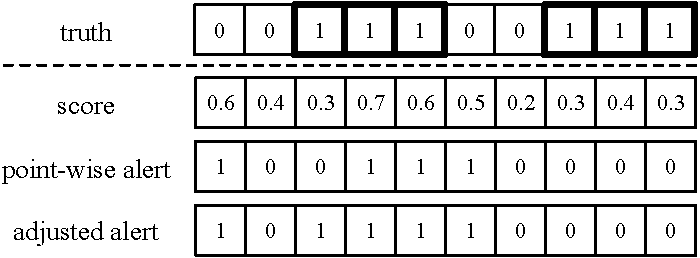
\includegraphics[width=0.9\textwidth]{fig/label_calculate.pdf}\\
%       \end{minipage}
%       %\vspace{-5 mm}
%       \caption{Illustration of the strategy for modified metrics. The first row is the truth with 10 contiguous points and two anomaly segments highlighted in the shaded squares. The detector scores are shown in the second row. The third row shows the point-wise detector results with a threshold of 0.5. The forth row shows the detector results after adjustment. We shall get precision 0.6, and recall 0.5. From the third row, the alert delay for the first segment is 1 interval (5 minute)~\cite{xu2018unsupervised}.
%       }
%       \label{fig:label_calculate}
%      % \vspace{-1 mm}
% \end{figure}

As is with~\cite{xu2018unsupervised}, we apply the \emph{best F-score} as the metric to evaluate anomaly detection methods.
The best F-score indicates the best possible performance of an anomaly detection method on a particular testing set, given an optimal global threshold. 
In practice, the best F-score is mostly consistent with Area Under the (ROC) Curve (AUC).

Note that in Section~\ref{subsec:overall-performance} and Section~\ref{subsec:effects_of_techniques}, we tune aThld based on the labels of the testing set (namely, the back 40\% of every new KPI stream) to obtain the \emph{best F-score}.
Although it is not entirely practical in real-world applications, it fully compares the \emph{best} performance of \name{}, iForest, Donut, Opprentice and the combination of ROCKA and Opprentice.
% It gives the best performance of \name{} on our test set on the global view, which is equivalent to AUC or PRC, but has a explicit practical meaning.
% In the classification problem, papers often use AUC or PRC to evaluate the performance of the algorithm. 
% In anomaly detection, we sample some thresholds in the threshold space and use the \textbf{best F-score} as the metric. It  
% Please note, we choose threshold from the train set and use it in test set to evaluate actual performance in Section~\ref{subsubsec:choose_threshold}, while the best F-core on the test set gives the optimal situation of the algorithm.

\subsection{Evaluation of The Overall Performance}
\label{subsec:overall-performance}
% The clustering result of ROCKA is shown in TABLE~\ref{table:rocka-results}. 
% We can see that ROCKA performs well on our KPI stream set. It groups all KPI streams into correct clusters. We just only apply this clustering algorithm and do not improve it.





% except for outliers. We will ignore these outliers in the next step. In addtion, ROCKA is easy to be parallelized when dealing with the large-scale KPI streams, it takes only just a few seconds to finish clustering. 

% \begin{table}
% \caption{Clustering result of ROCKA}
% \vspace{-0.5em}
% \label{table:rocka-results}
% \begin{center}
% \begin{tabular}{| c | r | r |}
% \hline
% \textbf{F-score} & \textbf{\# Clusters} & \textbf{Cost time(ms)} \\ \hline
% 1 & 5 & 6850 \\
% \hline
% \end{tabular}
% \end{center}
% % \vspace{-1.5em}
% \end{table}

To evaluate the performance of \name{} in anomaly detection for KPI streams, we calculate its best F-score, and compare it with that of iForest~\cite{ding2013anomaly}, Donut~\cite{xu2018unsupervised} and Opprentice~\cite{liu2015opprentice}.

% The above four methods have the following specific settings:
% \begin{itemize} 
%   \item \textbf{\name{}}. 
For each of the 81 new KPI streams, we train \name{} using the features extracted from the front 60\% of it, as well as the features and manual labels of its cluster centroid (KPI stream).
 Then we use this \name{} model to detect anomalies on the back 40\% of this new KPI stream.
As for iForest, Donut and Opprentice, we divide each new KPI stream (of the 81 KPI streams) into training set and testing set, whose ratios are (front) 60\% and (back) 40\%, respectively.
  % \item \textbf{iForest}. We divide each new KPI stream (of the 81 KPI streams) into training set and testing set, whose ratios are 60\% and 40\%, respectively.
  % \item \textbf{Donut}. The training processes is the same as above.
  % \item \textbf{Opprentice}. The split method is same as above. But the train set (60\% of each KPI stream) has label information.
  
% \end{itemize}

% In anomaly detection, we measure the best F-Score of \name{} to evaluate performacne, and compared it with Isolation Forest~\cite{liu2012isolation}, Donut~\cite{xu2018unsupervised} and Opprentice~\cite{liu2015opprentice} which have be discussed in Section~\ref{sec:related}
% two selected algorithms.
% \begin{itemize}
%   \item Isolation Forest~\cite{liu2012isolation} is a representative unsupervised anomaly detection model. It assumes that the anomaly points are few and different, then constructs tree structure to separate the points from the rest of points until all are isolated. The points closer to the root of the tree will be regared as anomaly points while the normal points are always at the bottom of the tree. This method is simple and efficient, and does not require any sophisticated assumptions.
% 	\item Opprentice~\cite{liu2015opprentice} is a state-of-art supervised method. It ensemble 14 widely-used traditional statistical algorithms~\cite{knorn2008adaptive, lu2009network, pincombe2005anomaly, chen2013provider, yan2012argus, mahimkar2011rapid, lee2012threshold,krishnamurthy2003sketch} with 133 enumerated configurations of hyper-parameters for these algorithms to extract feature for the points. Then it trains classifier using Random Forest. Opprentice requires anomaly infomation of each curve. In our experiments, we renounce the detectors that take too long to initialize(\EG{}, TSD~\cite{chen2013provider} needs at least 1 week) and extract 106 feature for one point.
% \end{itemize}
\begin{figure}
% \setlength{\abovecaptionskip}{-0.03cm}
      \begin{minipage}[h]{1.0\linewidth}
      \centering
      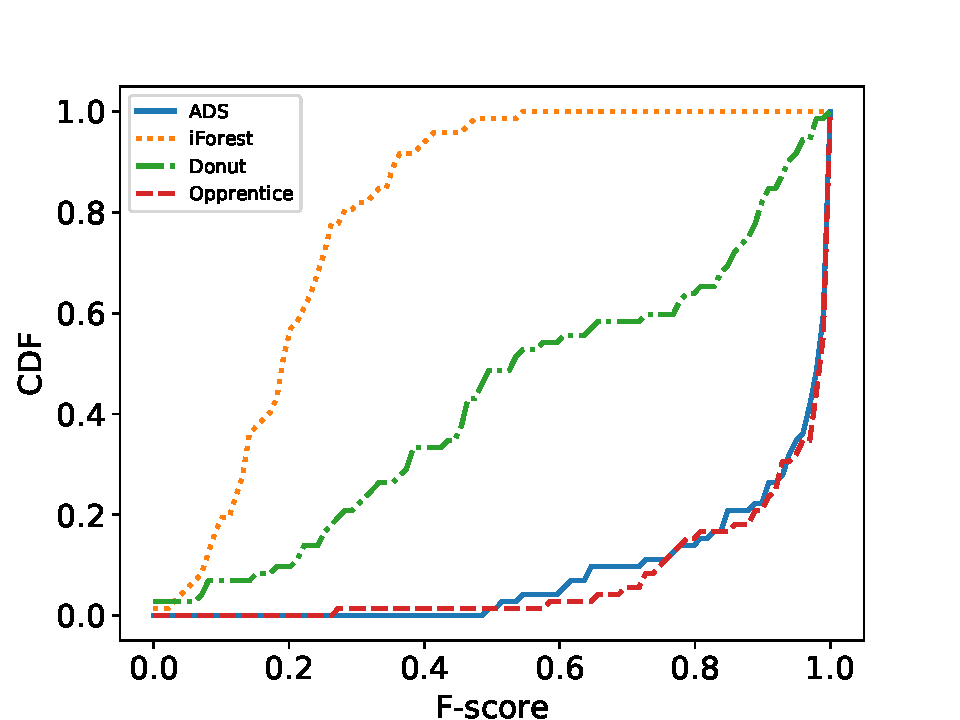
\includegraphics[width=0.9\textwidth]{fig/overview_fscore.pdf}\\
      \end{minipage}
      %\vspace{-5 mm}
      \caption{CDFs of the best F-scores of each new KPI stream using \name, iForest, Donut and Opprentice, respectively.
      }
      \label{fig:overview_fscore}
      \vspace{-6 mm}
     % \vspace{-1 mm}
\end{figure}

Figure~\ref{fig:overview_fscore} shows the cumulative distribution functions (CDFs) of the best F-scores of each KPI stream (of the new 81 KPI streams) using the above four methods.
Note that in this CDF figure, being closer to the upper left means worse performance, and being closer to the bottom right means better performance.
We can see that both \name{} and Opprentice perform superior in detecting anomalies for KPI streams, with 80\% of best F-scores over 0.8.
 Their performance is much better than that of iForest and Donut, for the following reasons: 
 (1) iForest is
 % cannot effectively extract features (traditional statistical anomaly detection algorithms and their parameters) from KPI streams, and it is 
 sensitive to noises in the training set because it does not utilize any labels~\cite{ding2013anomaly}. 
 (2) Donut is a deep Bayesian model, which requires a lot of training data to get good results (say six months worth of KPI streams)~\cite{xu2018unsupervised}.
However, as Table~\ref{table:game-related-KPI} shows, we have to train the model using 60\% of one month, namely 18 days, worth of newly emerging KPI streams, which is a too small amount of training data for Donut.

 % which is infeasible for the newly emerging KPI streams.
 % However, our scenario often requires algorithms to performance well within a month. Donut can't handle this task whose training data is very scarce.



\begin{table*}
\caption{Average best F-scores of \name, iForest, Opprentice, Donut and ROCKA+Opprentice in the five clusters, respectively}
% \vspace{-0.5em}
\label{table:average_fscore}
\begin{center}
\begin{tabular}{| c | c | c | c | c | c | c |}
\hline
\textbf{Cluster} & \textbf{\tabincell{l}{\# KPI streams}} &\textbf{\name{}} & \textbf{iForest} & \textbf{Donut} & \textbf{Opprentice} & \textbf{\tabincell{l}{ROCKA + Opprentice}}  \\ \hline
A & 7 & 0.91 & 0.33 & 0.42 & 0.90 &0.67   \\ \hline
B & 9 & 0.91 & 0.21 & 0.37 & 0.91 &0.88  \\ \hline
C & 8 & 0.95 & 0.22 & 0.28 &0.98 &0.94  \\ \hline
D & 53 & 0.93 & 0.19 & 0.67 &0.94 &0.90  \\ \hline
E & 4 & 0.67 & 0.13 & 0.45 &0.71 &0.66  \\ \hline
Overall &81 & 0.92  & 0.20 & 0.57 &0.93 &0.87   \\
\hline
\end{tabular}
\end{center}
\vspace{-6 mm}
% \vspace{-1.5em}
\end{table*}



% Please note that the whole cluster centroids will participate in training, so we don't evaluate the performance on these cluster centroids. 
To intuitively compare the best F-scores of \name, iForest, Opprentice and Donut, we list the average best F-scores of the above four methods on the five clusters in TABLE~\ref{table:average_fscore}, respectively.
\name{} and Opprentice perform well across all the five clusters and much better than iForst and Donut, demonstrating that it is important to utilize anomaly labels in anomaly detection for newly emerging KPI streams.
Specifically, \name~improves the average best F-score by 61.40\% (as opposed to Donut) to 360\% (as opposed to iForest).



% and the number of labelled KPI used in training of above four experiments for each KPI stream cluster. 
% Fig.~\ref{fig:overview_fscore} gives the cumulative distribution function (CDF) of best F-score of each KPI stream. 

% We can see that, \name{} achieves the outstanding performance on most of the KPI streams with an average best F-score of 0.92 on 81 KPI streams, 80\% KPI streams has a F-score over 0.8 which far exceeds iForest with an average of 0.20 and Donut with an average of 0.57. 


 % The supervised method Opprentice also performs well, but \name{} uses only five labelled centroids, which reduces 94\% cost of data labelling. The experiment result shows that \name{} is of high practical value, it can free operators from the heavy work of data labelling while ensuring outstanding performance. In reality, the amount of KPI streams is far more than our KPI stream set which means the cost reduction of \name{} will be more meaningful.

Although the supervised learning based method, Opprentice, performs similarly to \name, it needs much more labeling works.
For example, in this setting, \name~is trained based on only \emph{five} labeled KPI streams on cluster centroids, while Opprentice is trained using all the $81$ labeled KPI streams.
As aforementioned, over 6000 new KPI streams are produced per 10 days in the studied online gaming service. 
Manually labeling all the newly emerging KPI streams to detect KPI anomalies is infeasible in practice.
Consequently, Opprentice is not appropriate for our scenario. 


\subsection{Evaluation of CPLE}
\label{subsec:effects_of_techniques}
To the best of our knowledge, this is the first work to apply semi-supervised learning to the KPI anomaly detection problem. 
We adopt a robust semi-supervised learning model, CPLE, which is suitable for KPI anomaly detection and only requires \textit{similar} (not necessarily \textit{the same}) data distribution between the existing labeled KPI stream and the new KPI stream. 

To evaluate the performance of CPLE, we compare the performance of \name{}, which is the combination of ROCKA and CPLE, to that of the combination of ROCKA and a state-of-art supervised learning method -- Opprentice~\cite{liu2015opprentice} (ROCKA + Opprentice henceforth). 
We set up ROCKA + Opprentice as follows.
We first apply ROCKA to group the 70 historical KPI streams into five clusters, and classify the 81 new KPI streams into these clusters.
% For each of the 81 new KPI streams, we train Opprentice using the features and manual labels of its cluster centroid.
For each cluster, we train Opprentice using the features and manual labels of its centroid KPI streams.
After that, we detect anomalies for the back 40\% of each new KPI stream using the Opprentice model trained based on this new KPI stream's cluster centroid.
% the KPI stream on the centroid of the cluster that the new KPI stream belongs to.
% In addition, we test \name{} based on the manual labels of the back 40\% of each new KPI stream.

% The model only trained on the centroids. 
% Firstly we apply ROCKA to group the 86 KPI streams into clusters. Then, we train a Opprentice model only on the whole labelled centroid in each cluster, then we use this model to detect anomalies on the 40\% of other KPI streams belonging to the same cluster. 
% Finally, we get the best F-score of each KPI stream, and compare with \name{}. 

% In this section, We conduct additional experiments to show the effects of semi-supervised Learning method CPLE.
% \begin{itemize}
%   \item ROCKA+CPLE. It's our \name{}.
%   \item 
% \end{itemize}


% Fig.~\ref{fig:contrast_fscore} gives the cumulative distribution function (CDF) of best F-score of each KPI stream. 
% \begin{table}
% \caption{Average best F-score for anomaly detection of \name{} and ROCKA+Opprentice }
% % \vspace{-0.5em}
% \label{table:contrast_fscore}
% \begin{center}
% \begin{tabular}{| c | r | r | r |}
% \hline
% \textbf{Cluster} & \textbf{\name{}} & \textbf{ROCKA+Opprentice} & \textbf{\# KPI streams} \\ \hline
% A & 0.91 & 0.67 & 7 \\ \hline
% B & 0.90 & 0.88 & 9 \\ \hline
% C & 0.95 & 0.94 & 8 \\ \hline
% D & 0.93 & 0.90 & 53 \\ \hline
% E & 0.67 & 0.66 & 4 \\ \hline
% Overall & 0.92 & 0.87 &  \\
% \hline
% \end{tabular}
% \end{center}
% \vspace{-1.5em}
% \end{table}

% \begin{figure}
%       \begin{minipage}[h]{1.0\linewidth}
%       \centering
%       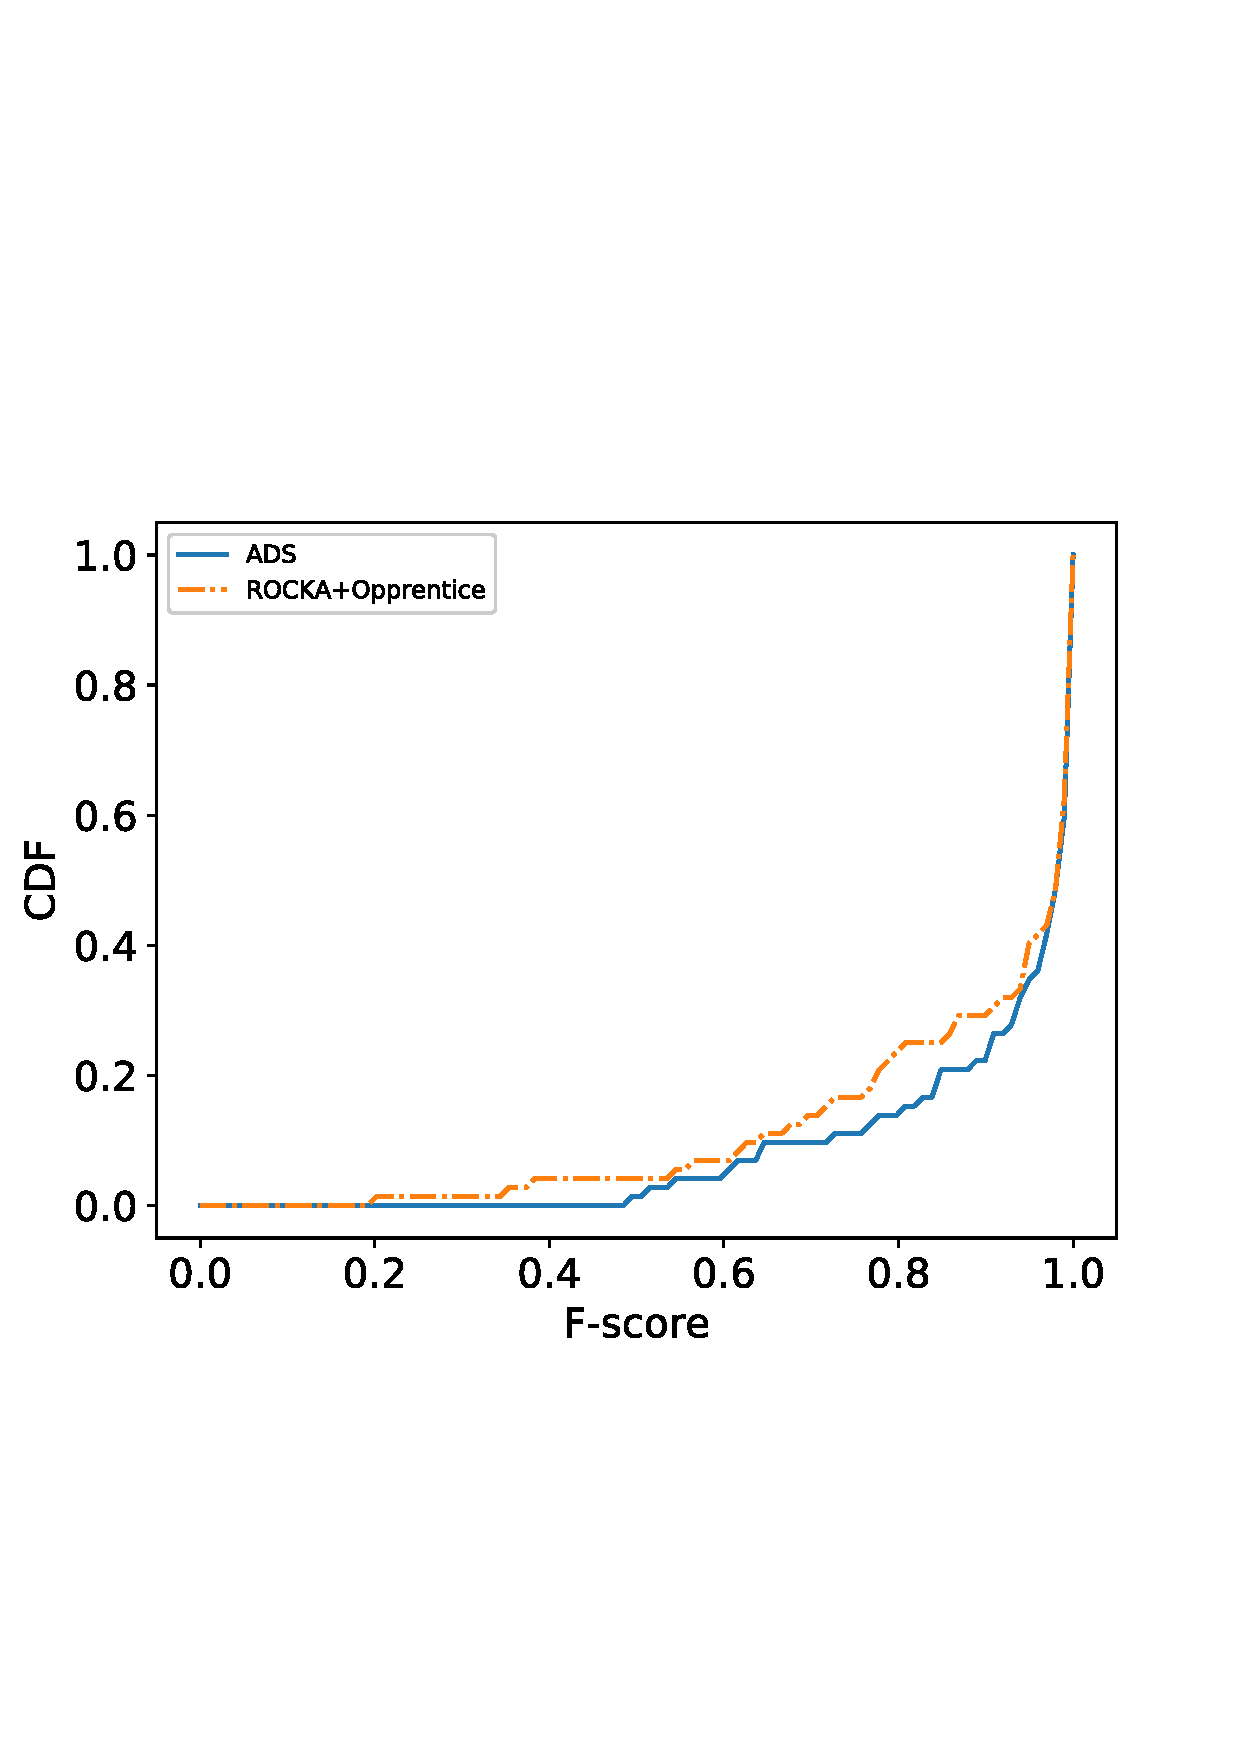
\includegraphics[width=0.9\textwidth]{fig/contrast_fscore.pdf}\\
%       \end{minipage}
%       %\vspace{-5 mm}
%       \caption{CDF of best F-score on each KPI stream of \name{} and ROCKA+Opprentice
%       }
%       \label{fig:contrast_fscore}
%      % \vspace{-1 mm}
% \end{figure}

\begin{table}
\caption{ The new KPI streams where \name{} performs significantly better than ROCKA + Opprentice }
% \vspace{-0.5em}
\label{table:difference_fscore}
\begin{center}
\begin{tabular}{| c | c | c |}
\hline
\textbf{KPI stream ID} & \textbf{\name{}} & \textbf{ROCKA + Opprentice} \\ \hline
$\alpha$ & 0.86 & 0.62 \\ \hline
$\beta$ & 0.91 & 0.20 \\ \hline
$\gamma $ & 0.72 & 0.46 \\ \hline
$\delta $ & 0.80 & 0.55 \\ \hline
... & ... & ... \\
\hline
\end{tabular}
\end{center}
\vspace{-6 mm}
% \vspace{-1.5em}
\end{table}

TABLE~\ref{table:average_fscore} compares the average best F-scores of \name{} and ROCKA + Opprentice on each cluster. 
We can see that \name{} outperforms ROCKA + Opprentice on every cluster, and greatly outperforms it by 35.82\% on cluster A. 
% Specific to A cluster, the performance improvement will be more obvious. 
TABLE~\ref{table:difference_fscore} lists the new KPI streams where \name{} performs significantly better than ROCKA + Opprentice, and the best F-scores of the above two methods on these KPI streams, respectively.

\begin{figure}
\setlength{\abovecaptionskip}{-0.1cm}
      \begin{minipage}[h]{1.0\linewidth}
      \centering
      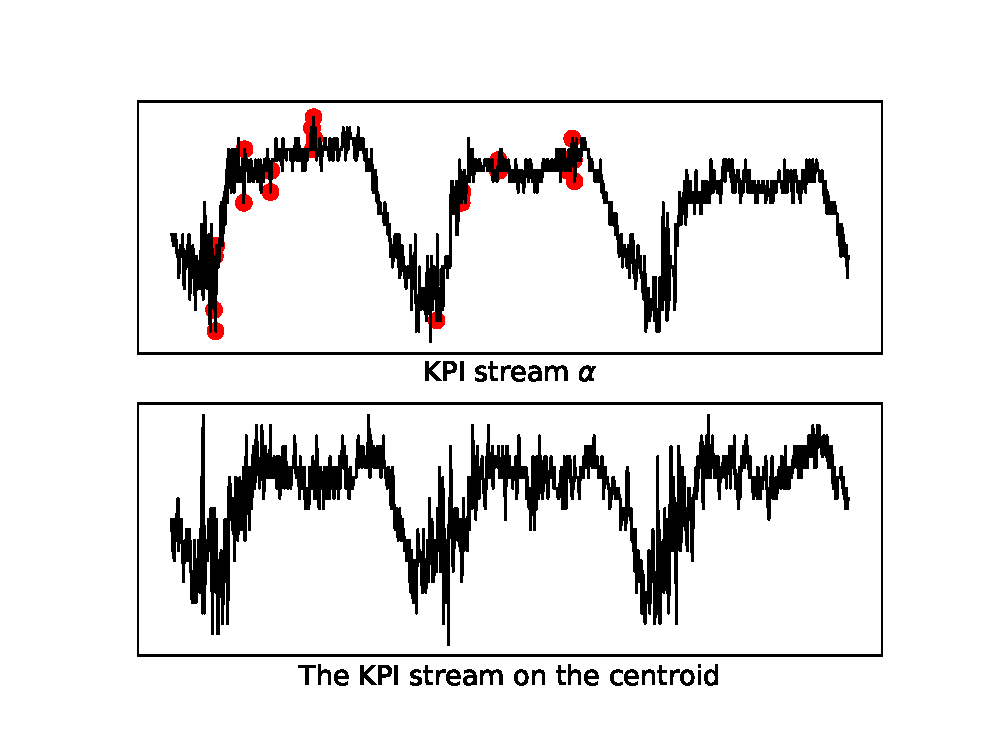
\includegraphics[width=0.9\textwidth]{fig/kpi_evaluation.eps}\\
      \end{minipage}
      %\vspace{-5 mm}
      \caption{The anomaly detection results of ROCKA + Opprentice on KPI stream $\alpha$, and $\alpha$'s cluster centroid KPI stream.
      The red data points are anomalous determined by ROCKA + Opprentice while in actual they are normal.
      }
      \label{fig:centroid_and_curve}
      \vspace{-6 mm}
     % \vspace{-1 mm}
\end{figure}

Here we explain why \name{} performs better than ROCKA + Opprentice.
KPI stream clustering methods such as ROCKA usually extract baselines (namely underlying shapes) from KPI streams and ignore fluctuations.
% The main reason is that, in order to calculate distance, ROCKA ignore the fluctuations and uses moving average to extract underlying shape of each KPI stream called baseline which will be taken as input to clustering algorithm. 
However, the fluctuations of KPI streams can impact anomaly detection.
% But the fluctuations count much in anomaly detection. 
For example, Figure~\ref{fig:centroid_and_curve} shows the new KPI stream $\alpha$, and the KPI stream on the its cluster centroid.
KPI stream $\alpha$ and the centroid KPI stream have very similar baselines, but they have different fluctuation degrees, which is not uncommon in practice.
This lead to that ROCKA + Opprentice, which is trained based only on the centroid KPI stream, generates a lot of false alarms.
% one curve 5-69 belonging to A cluster and it's centroid, the Opprentice result on it is 0.94, the \name{} results on it is 0.86, while the ROCKA+Opprentice on it is only 0.62. 
% 5-69 and it's centroid have similar baseline but vary by their fluctuations severity levels which is very common in reality. 
% Under this circumstance, the model trained by only centroid performs extremely bad. We can see that ROCKA+Opprentice determines too many normal points as anomaly points which reduces the precision.

\name{} addresses the above problem effectively using semi-supervised learning. 
In other words, it learns not only from the labels of the centroid KPI stream, but also from the fluctuation degree of the new KPI stream.
This is consistent with the observation that the model trained based on both labeled and unlabeled data should not be worse than the one trained based only on the labeled data~\cite{loog2016contrastive}.

The experiment results strongly demonstrate \name{}'s robustness in KPI anomaly detection.
% First, we get the initial model on the labelled centroid. Then, in the process of training, the model is constantly adapting to the KPI stream until finish training. 
% It not only utilizes the label information on the centroid, but also the fluctuation severity level on the KPI stream to get a satisfactory result. 
% CPLE guaranteed that . 
% If the KPI stream and it's centroid vary by their fluctuations severity levels, CPLE will continuously train to improve performance, if not, CPLE will converge very quickly and also performs well. 


% \begin{figure}
%   \begin{subfigure}[t]{0.5\columnwidth}
%     \centering
%     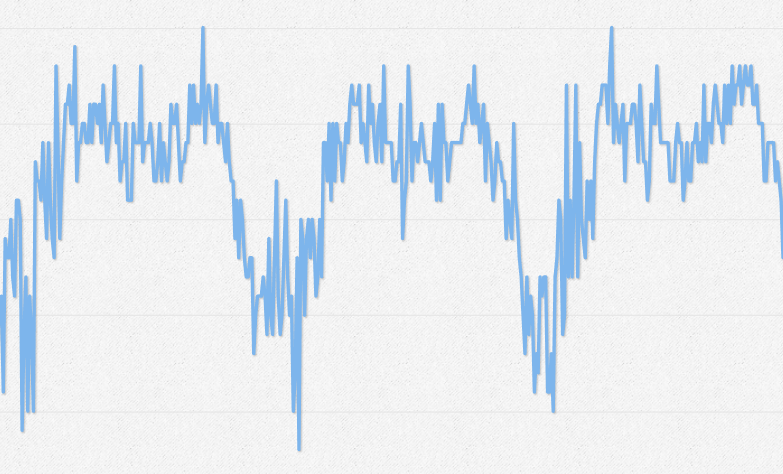
\includegraphics[width=.9\linewidth,height=28mm]{fig/medios.png}
%   \vspace{0.2em}
%     \caption{The centroid of cluster A}\label{fig:centroid}
%   \end{subfigure}\hfill
%   \begin{subfigure}[t]{0.5\columnwidth}
%     \centering
%     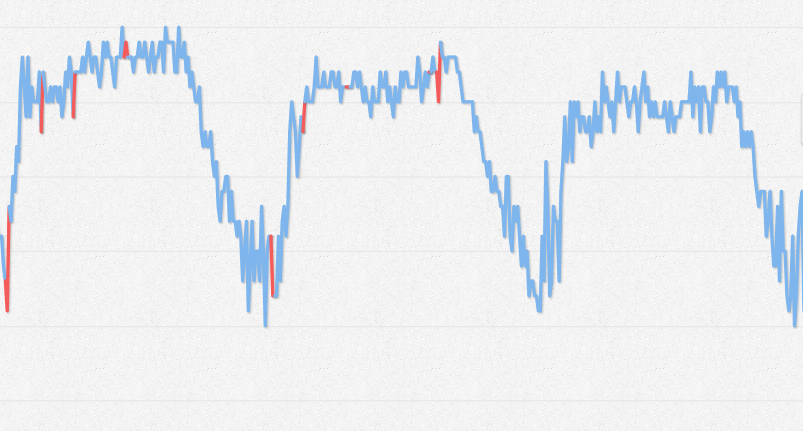
\includegraphics[width=.9\linewidth,height=28mm]{fig/5_69.png}
%   \vspace{0.2em}
%     \caption{The detection results of one curve belonging to cluster A with ROCKA+Opprentice}\label{fig:5_69}
%   \end{subfigure}
%   \caption{The detection results of one curve with ROCKA+Opprentice and it's centroid. The rea lines are anomaly points determined by the algorithm, but normal points in reality.
%   }
%   \label{fig:centroid_and_curve}
%     % \vspace{-1.2em}
% \end{figure}



% \subsection{Evaluation of aThld}
% \label{subsec:choose_threshold}
% % As of now, we have demonstrated the advantages of \name{} using best F-score in detail.
%  % However, for our system can be applied in practice, we also need to choose a the appropriate threshold from train data. 
%  % Only the point whose anomaly score given by \name{} exceeds the threshold will be regard as an anomaly point. 
%  As aforementioned, we tune aThld based on the labeling information of the testing set in order to calculate the best F-score.
%  However, it is infeasible in practice, because we cannot label the new testing set, \emph{i.e.,} the newly emerging KPI streams.
%  As discussed in Section~\ref{subsubsec:choose_threshold}, aThld can be set based on either the F-score of the labeled KPI stream (labeled-aThld henceforth), or the elbow point of the unlabeled one (unlabeled-aThld henceforth).
%  Here we compare the performance of the above two methods using the following settings.
%  % We measure the best F-score of \name{} and compared it with two ways to choose threshold as described earlier in Section~\ref{subsubsec:choose_threshold}.
% \begin{itemize}
%   \item \textbf{Labeled-aThld}. 
%   For each of the new 81 KPI streams, we set its aThld as the one that maximizes the F-score of the centroid KPI stream of the cluster where this new KPI stream belongs.
%   % We choose the threshold which maximizes the F-score on the labeled data of train.
%   \item \textbf{Unlabeled-aThld}. 
%   For each new KPI stream, we tune its aThld using the elbow point of CDF curve of the front 60\% data points' severity of this KPI stream.
%   % We choose the threshold by Elbow Point on the unlabelled data of train.
% \end{itemize}

% \begin{figure}
%       \begin{minipage}[h]{1.0\linewidth}
%       \centering
%       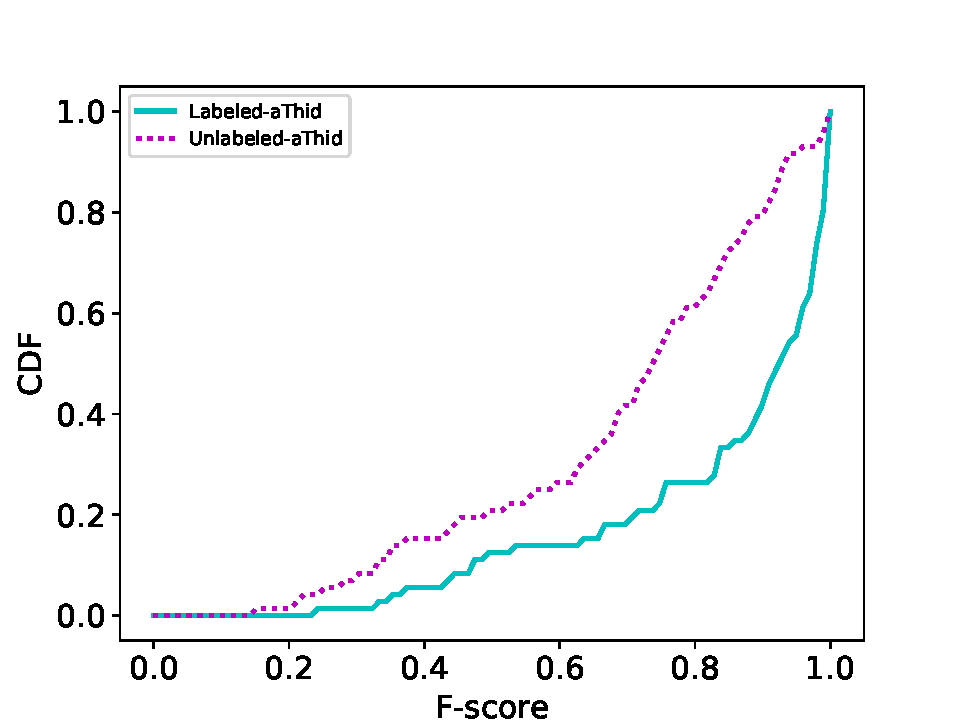
\includegraphics[width=0.9\textwidth]{fig/choose_thre.pdf}\\
%       \end{minipage}
%       %\vspace{-5 mm}
%       \caption{CDFs of the F-scores using labeled-aThld and unlabeled-aThld, respectively.
%       }
%       \label{fig:chooose_threshold}
%      % \vspace
% \end{figure}

% Figure~\ref{fig:chooose_threshold} shows the CDFs of the F-scores using labeled-aThld and unlabeled-aThld for 81 new KPI streams, respectively.
% Using labeled-aThld as the threshold tuning method achieves an average F-score of 0.84, which is much better than using unlabeled-aThld (the average F-score is 0.69).
% Therefore, we choose label-aThld rather than unlabeled-aThld to tune threshold for \name{}.
% Based on an on-site investigation, operators are quite satisfactory with the result achieved by label-aThld.


% Figure~\ref{fig:chooose_threshold} shows experiments' results. The average of best F-score of \name{} is 0.92, the E1 gets average 0.84 F-score, while the E2 gets only average 0.69 F-score. 
% We can determine the conclusion that E1 is the most suitable methods to choose threshold in \name{}. With the label information, E1 can find the right threshold more easily. In addtion, the experiments indicate that \name{} is of high practical value, and can be applied in real online detection with average F-score 0.84.
% {-1 mm}